\def \kaflanr {17}
\lecture[\kaflanr]{\kaflanr. Vigursvið og stigulsvið}{lecture-text}
\date{2.~mars 2015}
\newcounter{mycount}
\refstepcounter{mycount}

\begin{document}

\subsection{}
	\maketitle





\subsection{Vigursvið} 

\subsubsection{Skilgreining \kaflanr.\arabic{mycount}}\stepcounter{mycount}
 {\em Vigursvið} á $\R^2$ er vörpun
$$\Fv(x,y)=F_1(x,y)\,\iv+F_2(x,y)\,\jv.$$
Þegar talað er um vigursvið þá hugsum við vigurinn $\Fv(x,y)$ sem vigur í
$\R^2$ sem hefur fótpunkt í punktinum $(x,y)$.   

 \medskip
Vigursvið $\Fv(x,y)=F_1(x,y)\iv+F_2(x,y)\jv$ er sagt {\em samfellt} ef
föllin $F_1(x,y)$ og $F_2(x,y)$ eru samfelld.

\medskip
Vigursvið á $\R^3$ er vörpun 
$$\Fv(x,y,z)=F_1(x,y,z)\,\iv+F_2(x,y,z)\,\jv+F_3(x,y,z)\,\kv.$$
Við hugsum $\Fv(x,y,z)$ sem vigur með $(x,y,z)$ sem fótpunkt.
  Skilgreiningin á því að
vigursvið í $\R^3$ sé samfellt er eins og á samfeldni vigursvið í
$\R^2$ . 





\subsection{Vigursvið}
 \begin {figure}[h!]
 \centering
            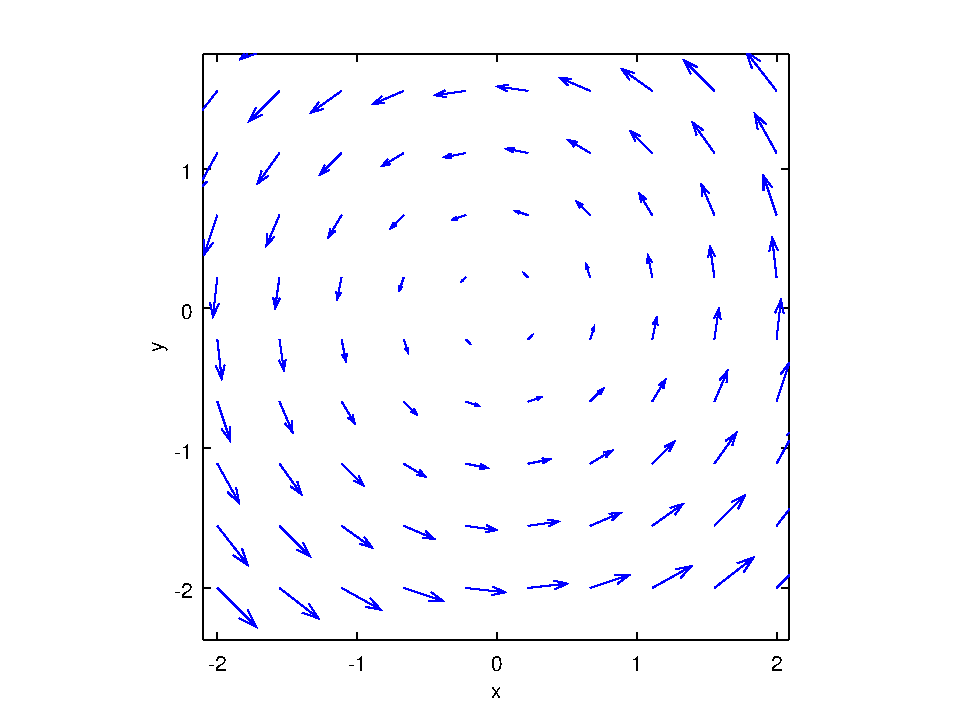
\includegraphics[width=0.75\linewidth]{vfield}
            \caption*{ Vigursviðið $\mathbf{F}(x,y) = -y\iv + x \jv$.}
\end {figure}






\subsection{Straumlína} 

\subsubsection{Skilgreining \kaflanr.\arabic{mycount}}\stepcounter{mycount}
 Ferill $C$ í planinu kallast {\em straumlína}
(e.~stream line, flow line)
fyrir vigursvið $\Fv(x,y)$ ef í hverjum punkti $(x,y)$ á ferlinum er
vigurinn $\Fv(x,y)$ snertivigur við ferilinn. 


 \begin {figure}[h!]
 \centering
            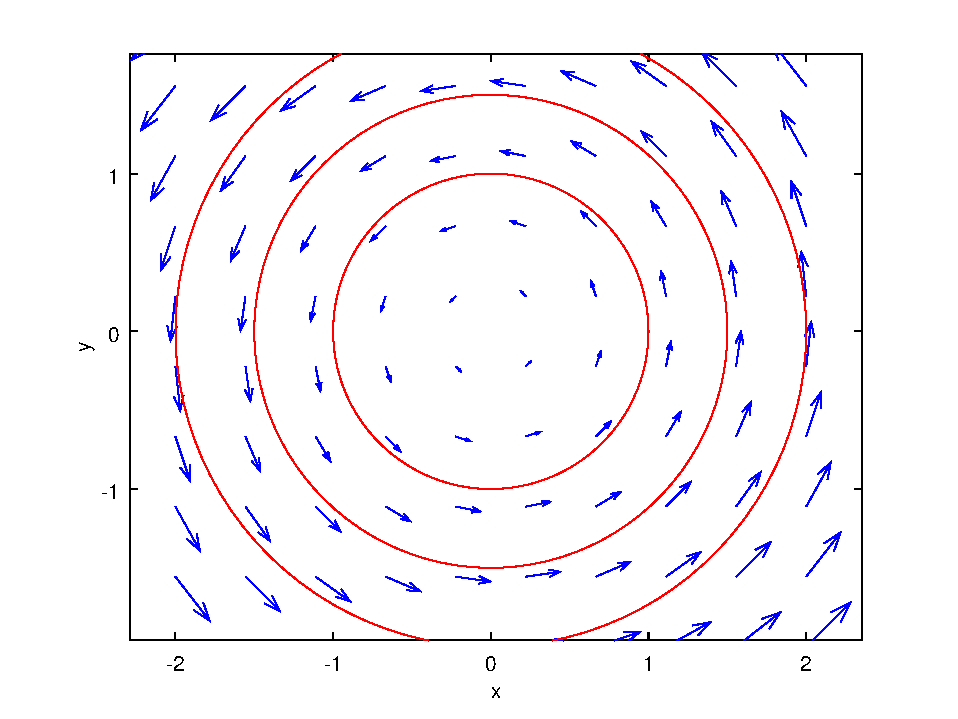
\includegraphics[width=0.55\linewidth]{flowlines}
            \caption*{ Vigursviðið $\mathbf{F}(x,y) = -y\iv + x \jv$ ásamt nokkrum straumlínum.}
\end {figure}




\subsection{Stigulsvið} 

\subsubsection{Skilgreining \kaflanr.\arabic{mycount}}\stepcounter{mycount}
Vigursvið $\Fv(x,y)$ kallast {\em stigulsvið} eða {\em geymið svið}
(e.~gradient field, conservative  field) á mengi $D$ ef til er fall $\phi(x,y)$ þannig að $$\Fv(x,y)=\nabla\phi(x,y)$$ fyrir alla punkta $(x,y)\in D$, það er að segja ef 
$$\Fv(x,y)=F_1(x,y)\,\iv+F_2(x,y)\,\jv$$ þá er $$F_1(x,y)=\frac{\partial}{\partial x}\phi(x,y) \quad \text{og}\quad  F_2(x,y)=\frac{\partial}{\partial y}\phi(x,y).$$

Vigursvið $\Fv(x,y,z)$ kallast {\em stigulsvið} eða  {\em geymið svið} ef til er fall $\phi(x,y,z)$ þannig að $\Fv(x,y,z)=\nabla\phi(x,y,z)$. 

\medskip
Fallið $\phi$ kallast {\em mætti} (e.~potential) fyrir vigursviðið $\Fv$.






\subsection{} 

\subsubsection{Setning \kaflanr.\arabic{mycount}}\stepcounter{mycount}
 Látum $\Fv(x,y)=F_1(x,y)\,\iv+F_2(x,y)\,\jv$ vera vigursvið þannig að föllin $F_1(x,y)$ og $F_2(x,y)$ hafi samfelldar hlutafleiður.  Ef $\Fv(x,y)$ er stigulsvið þá er 
$$\frac{\partial}{\partial y}F_1(x,y)=
\frac{\partial}{\partial x}F_2(x,y).$$

\smallskip

{\bf Athugasemd.}  Þó að hlutafleiðurnar séu jafnar
þá er {\bf ekki} hægt að álykta að $\Fv$ sé stigulsvið.  Þetta
atriði verður rætt síðar.
 





\subsection{} 

\subsubsection{Setning \kaflanr.\arabic{mycount}}\stepcounter{mycount}
Látum
$\Fv(x,y,z)=F_1(x,y,z)\,\iv+F_2(x,y,z)\,\jv+F_3(x,y,z)\,\kv$ vera vigursvið
þannig að föllin $F_1(x,y,z), F_2(x,y,z)$ og $F_3(x,y,3)$ hafi
samfelldar hlutafleiður.  Ef $\Fv(x,y,z)$ er stigulsvið þá er  

\begin {align*}
\frac{\partial}{\partial y}F_1(x,y,z) &=
\frac{\partial}{\partial x}F_2(x,y,z), \\
\frac{\partial}{\partial z}F_1(x,y,z) &=
\frac{\partial}{\partial x}F_3(x,y,z) \quad \text{og} \\
\frac{\partial}{\partial z}F_2(x,y,z)&=
\frac{\partial}{\partial y}F_3(x,y,z).
\end {align*}








\subsection{} 

\subsubsection{Reikniaðferð \kaflanr.\arabic{mycount}}\stepcounter{mycount}
 Finna á mætti $\phi(x,y)$ fyrir stigulsvið  $\Fv(x,y)=F_1(x,y)\,\iv+F_2(x,y)\,\jv$.  Viljum finna fall $\phi(x,y)$ þannig að 
$$\frac{\partial}{\partial x}\phi(x,y)=F_1(x,y)\qquad
\mbox{og}\qquad \frac{\partial}{\partial y}\phi(x,y)=F_2(x,y).$$
 Með því að heilda þessar jöfnur fæst að 
 $$\phi(x,y)=\int F_1(x,y)\,dx+C_1(y)$$
og
$$\phi(x,y)=\int F_2(x,y)\,dy+C_2(x).$$
Þegar fyrra stofnfallið er reiknað þá er $y$ hugsað sem fasti og því fæst heildunarfasti sem getur verið fall af $y$.  Lokaskrefið er  svo að horfa á jöfnurnar tvær hér að ofan og sjá hvort ekki er hægt að finna gildi fyrir heildunarfastanna $C_1(x)$ og $C_2(y)$ þannig að sama formúlan fyrir $\phi(x,y)$ fáist.  




\end{document}